\subsubsection{Qwen Sparse Attention}
\label{sec:qsa}

\paragraph{Motivation.}
% Background
By selectively attending to important context, sparse attention alleviates the quadratic computational bottleneck of softmax attention in long-context scenarios.
% DSA Indexer
Recently, DSA~\citep{liu2025deepseek} has achieved considerable inference speedups using a lightweight indexer to generate token-level sparse masks.
% Indexer weakness
However, as sequence length increases, the overhead of its $O(n^2)$ indexer remains non-negligible.

\begin{figure}[h]
    \centering
    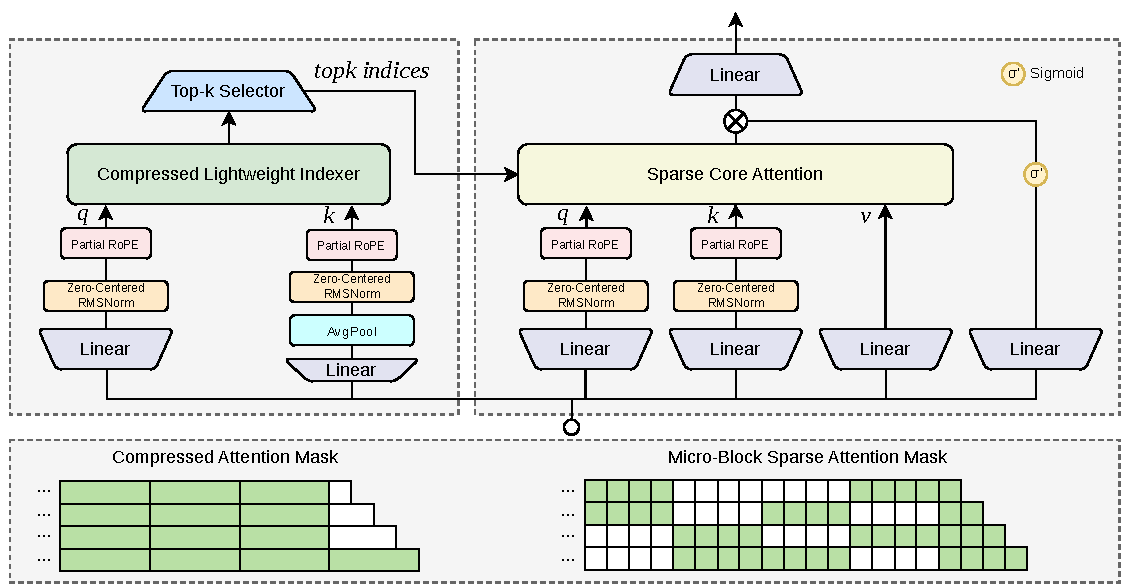
\includegraphics[width=\linewidth]{figs/qsa_arch.pdf}
    \caption{Overview of Qwen Sparse Attention (QSA). The QSA indexer (left) uses a compressed causal attention mask to score key blocks and select the top-$k$ indices. 
    These indices are expanded into a micro-block sparse attention mask for sparse core attention (right).}
    \label{fig:qsa_arch}
\end{figure}

% Qwen3.8-Flash-Next
To reduce this indexing cost, Qwen3.8-Flash-Next adopts Qwen Sparse Attention (QSA).
% Micro-Block
Specifically, QSA employs a lightweight indexer that compresses the sequence into micro-block representations, estimates their importance, and selects the most relevant context for attention computation.
% impact
This design reduces indexing overhead on long inputs while balancing task performance and inference efficiency.
% Hybrid model
Compared with methods that share indices across layers, the within-layer sequence compression in QSA relies less on cross-layer similarity, making it naturally suited to hybrid architectures.

% Figure
Figure \ref{fig:qsa_arch} illustrates the QSA architecture. A compressed lightweight indexer first estimates context importance at micro-block granularity and then guides sparse computation in the core attention module.

\paragraph{Compressed Lightweight Indexer.}
% QK Proj (avg K)
Given an input hidden state $\mathbf{x}_i$, the indexer adopts an MQA~\citep{shazeer2019fast} with $H$ query heads and one shared key head.
It first applies independent lightweight projections:
\begin{equation}
    \widehat{\mathbf{q}}^h_i
    = \operatorname{RMSNorm}(\mathbf{W}^h_Q\mathbf{x}_i),
    \qquad
    \mathbf{k}_i=\mathbf{W}_K\mathbf{x}_i.
\end{equation}
% Key Avgpooling
To reduce the sequence length, keys are partitioned into non-overlapping blocks of $r$ tokens and compressed by average pooling.
Denoting the starting position of block $b$ by $p_b=b\cdot r$, the corresponding compressed key is
\begin{equation}
    \widehat{\mathbf{k}}_b
    = \operatorname{RMSNorm}\left(
        \operatorname{AvgPool}
        (\mathbf{k}_{p_b:p_b+r-1})
      \right),
    \qquad
    0\le b<\left\lfloor\frac{n}{r}\right\rfloor.
    \label{eq:qsa-avg-pooling}
\end{equation}
% RoPE embedding
For positional encoding, the indexer applies partial RoPE.
Specifically, partial RoPE is applied to 64 of the 128 dimensions in each indexer head, matching the rotary dimension used in the core attention module. 
% Thus, half of the indexer channels explicitly incorporate positional information through RoPE, while the remaining half is left unrotated.
As shown in Eq.~\eqref{eq:qsa-avg-pooling}, key compression is performed before positional encoding.
Each block is therefore first summarized into a content representation and then assigned a single block-level position.
This ordering avoids averaging token representations with different rotary phases.
Each query retains its token position $i$, whereas each compressed key is assigned the starting position $p_b$ of its block:
\begin{equation}
    \mathbf{q}_i^h
    = \operatorname{PRoPE}(\widehat{\mathbf{q}}_i^h, i),
    \qquad
    \bar{\mathbf{k}}_b
    = \operatorname{PRoPE}(\widehat{\mathbf{k}}_b, p_b).
    \label{eq:qsa-partial-rope}
\end{equation}
% relu QK (block causal mask)
Block-level importance scores $\mathbf{I}$ are then obtained through
block-causal scoring.
For query token $i$ and compressed block $b$,
ReLU-activated query--key similarities are summed over all indexer heads:
\begin{equation}
    I_{ib}
    =
    \left\{
    \begin{array}{cl}
        \displaystyle
        \sum_{h=1}^{H}
        \operatorname{ReLU}\left(
        \left\langle\mathbf{q}_i^h,\bar{\mathbf{k}}_b\right\rangle
        \right),
        & p_b+r-1\le i,\\[6pt]
        -\infty,
        & \text{otherwise},
    \end{array}
    \right.
    \label{eq:qsa-index-score}
\end{equation}
This block-causal condition allows each query to score only blocks that have been fully observed.
% TopK Block
Given a token budget $K$, each query selects the highest-scoring compressed blocks.
Since each block contains $r$ tokens, the block budget is
$K_B=\lceil K/r\rceil$:
\begin{equation}
    \mathcal{B}_i
    = \operatorname{TopK}_{K_B}\left(\{I_{ib}\}_b\right),
    \qquad
    K_B=\left\lceil\frac{K}{r}\right\rceil.
    \label{eq:qsa-topk-blocks}
\end{equation}
% topk expand
Selected blocks are then expanded to their original token indices and
truncated to the budget $K$.
Together with the tokens in the final incomplete
block, which are always included, they form the final set used for core attention computation.

\paragraph{Training Details.}
% Two Stage from CPT
QSA is introduced during the continued pretraining (CPT) stage of
Qwen3.8-Flash-Next with a sequence length of 256K tokens.
The training procedure consists of two stages: dense distillation and sparse training.
\begin{itemize}[leftmargin=1.5em]
\item \textbf{Stage 1: Dense Distillation.}
% Training detials
We first distill the full-sequence attention distribution of the backbone into the indexer.
% maxpooling
The token-level teacher distribution is obtained by summing the softmax attention distributions over all teacher heads and applying $L_1$ normalization.
Denoting the resulting probability from query $i$ to token $j$ by $a_{ij}$, the full token-level distribution is $\mathbf{a}_i\in\mathbb{R}^{n}$.
Following prior work~\citep{gao2024seerattention,wang2026proxyattn},
we apply max pooling to align this distribution with the block-level indexer scores, 
thereby preserving salient token-level signals that could otherwise be diluted during aggregation:
\begin{equation}
\bar{a}_{ib}
= \operatorname{MaxPool}(\mathbf{a}_{i,\,p_b:p_b+r-1}),
\qquad
\hat{\mathbf{a}}_{i}
= \frac{\bar{\mathbf{a}}_{i}}
{\lVert\bar{\mathbf{a}}_{i}\rVert_1}.
\label{eq:qsa-teacher-pooling}
\end{equation}
% KL
Letting $B=\lfloor n/r\rfloor$, the pooled teacher distributions $\hat{\mathbf{a}}_i\in\mathbb{R}^{B}$ and the indexer scores $\mathbf{I}_i\in\mathbb{R}^{B}$ share the same block dimension.
The normalized teacher scores are distilled into the indexer by minimizing
\begin{equation}
\mathcal{L}_{\mathrm{KL}}
= \frac{1}{N}\sum_i
  D_{\mathrm{KL}}\left(
      \hat{\mathbf{a}}_{i,:}
      \,\middle\Vert\,
      \operatorname{Softmax}(\mathbf{I}_{i,:})
  \right),
\label{eq:qsa-distillation-loss}
\end{equation}
where $N$ is the number of query tokens. Only complete key blocks are included in the KL loss for each query.
% hyper-param
During the warm-up stage, only the indexer is trained for 1,000 steps, using a learning rate of $1\times10^{-3}$.
Each step comprises $8$ sequences of 256K tokens, amounting to approximately 2B training tokens in total.

\item \textbf{Stage 2: Sparse Training.}
% Backgroud
After indexer initialization, the entire backbone is trained under the guidance of the indexer to adapt to sparse attention patterns.
% KL Loss (topk select)
Following Eq.~\eqref{eq:qsa-topk-blocks}, QSA first selects the top-$K_B$ blocks.
These blocks are expanded to token indices and combined with the tail tokens in the final incomplete block:
\begin{equation}
    \mathcal{S}_i
    = \operatorname{Expand}(\mathcal{B}_i)
      \cup
      \left\{r\left\lfloor\frac{i+1}{r}\right\rfloor,\ldots,i\right\}.
    \label{eq:qsa-token-set}
\end{equation}
The $\operatorname{Expand}$ operator maps the selected blocks to their token indices. The resulting set $\mathcal{S}_i$ is used for core attention computation. In this stage, the indexer KL loss is computed only over the top-$K_B$ blocks in $\mathcal{B}_i$.
Before evaluating the KL divergence, the teacher probabilities within $\mathcal{B}_i$ are renormalized to sum to one:
\begin{equation}
    \mathcal{L}_{\mathrm{KL}}
    = \frac{1}{N}\sum_i
      D_{\mathrm{KL}}\left(
          \hat{\mathbf{a}}_{i,\mathcal{B}_i}
          \,\middle\Vert\,
          \operatorname{Softmax}(\mathbf{I}_{i,\mathcal{B}_i})
      \right).
    \label{eq:qsa-stage2-kl}
\end{equation}
During the final stage of CPT, QSA is enabled and the backbone and indexer are jointly trained for 8,000 steps using a learning rate of $2.5\times10^{-5}$. Each step comprises $96$ sequences of 256K tokens, totaling roughly 200B training tokens.

\end{itemize}

\begin{figure}[t]
    \centering
    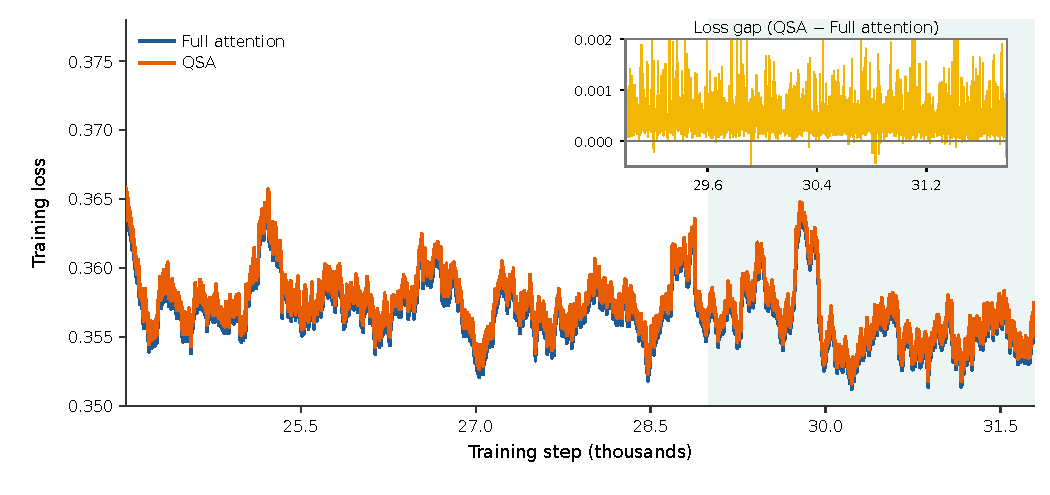
\includegraphics[width=0.93\linewidth]{figs/lm_loss_training_steps.pdf}
    \caption{Training LM loss with and without QSA. Curves are smoothed with a
    200-step moving average. The shaded region marks the final stage of
    continued pretraining, and the inset shows the per-step loss difference
    between QSA and the full-attention baseline in this region.}
    \label{fig:qsa-training-loss}
\end{figure}

\paragraph{Implementation Details.}
% scope
For Qwen3.8-Flash-Next, all full-attention layers in the backbone and MTP module are replaced with QSA to improve inference efficiency on long sequences.
% Indexer param
The compressed lightweight indexer adopts an MQA structure with four query heads and one shared key head, using the partial-RoPE configuration described above.
With a token budget of $K=2048$ and a compression ratio of $r=4$,
QSA selects up to $512$ complete blocks for each query
and additionally includes the tail tokens in the final incomplete block.
% Loss
Accurate importance estimates from the indexer enable the model to closely match the LM-loss trajectory of full attention during Stage 2 sparse training.
As shown in Fig.~\ref{fig:qsa-training-loss}, the two loss curves remain highly consistent,
with the overall loss difference on the order of $10^{-4}$.

% Training Kernel
For efficient training, we implement a fused QSA kernel that jointly computes sparse attention outputs and the KL loss without materializing intermediate results,
substantially reducing memory consumption.
The compressed indexer scores the sequence after compression, reducing both indexer computation and top-$k$ selection overhead. 
In addition, multi-step MTP reuses top-$k$ indices across prediction steps to further reduce draft-model inference costs.

\paragraph{Evaluation of QSA.}
% Setting
We evaluate QSA by comparing Qwen3.8-Flash-Next equipped with QSA against its full-attention baseline. Table~\ref{tab:qsa-pt-eval} reports the results across knowledge, STEM, reasoning, multilingual, and coding benchmarks,
providing a broad assessment of whether sparse attention affects the general capabilities of the model beyond long-context retrieval.
% PT Eval No significant loss
QSA matches or outperforms the full-attention baseline on seven of the eight benchmarks and improves the average score from 75.9 to 76.8.
The remaining differences are small and do not indicate systematic degradation in any task category.
% Conclusion
Overall, these results show that QSA preserves the general capabilities of the
model on short-context tasks while enabling more efficient long-context inference.


\begin{table*}[t]
\centering
\small
\caption{Model performance comparison between Qwen3.8-Flash-Next with full attention and QSA across widely used knowledge, STEM, reasoning, multilingual, and coding benchmarks. Bold values indicate the best result for each benchmark.}
\label{tab:qsa-pt-eval}
\resizebox{\textwidth}{!}{
\begin{tabular}{@{\extracolsep{\fill}}c cc cc c c cc c@{}}
\toprule
% \multirow{2}{*}{Method}
& \multicolumn{2}{c}{Knowledge}
& \multicolumn{2}{c}{STEM}
& \multicolumn{1}{c}{Reasoning}
& \multicolumn{1}{c}{Multilingual}
& \multicolumn{2}{c}{Code}
% & \multirow{2}{*}{Avg.} \\
& \\
\cmidrule(lr){2-3}
\cmidrule(lr){4-5}
\cmidrule(lr){6-6}
\cmidrule(lr){7-7}
\cmidrule(lr){8-9}
Method
& MMLU-Pro
& SuperGPQA
& MATH
& GSM8K
& BBH
& MMMLU
& EvalPlus
& MultiPL-E
& Avg. \\
\midrule
Full Attn & 72.9& 51.7& 69.8 & 91.0& 90.4
& \textbf{81.8}& 70.8& 78.4 & 75.9 \\
w/ QSA & \textbf{73.7}& \textbf{52.1}& \textbf{71.6} & \textbf{92.2}& \textbf{91.6} & 81.1& \textbf{72.3}& \textbf{79.8} & \textbf{76.8} \\
\bottomrule
\end{tabular}
}
\end{table*}

\begin{table*}[t]
\centering
\small
\caption{Long-context retrieval performance of Qwen3.8-Flash-Next on RULER and 8-needle MRCR.
RULER scores are averaged over sequence-length ranges. 
Bold values indicate the best result in each setting;
Avg. is the macro-average across the two benchmarks.}
\label{tab:qsa-long-context-eval}
\setlength{\tabcolsep}{4pt}
% \begin{tabular*}{\textwidth}{@{\extracolsep{\fill}}l cccc cccc c@{}}
\begin{tabular}{l cccc cccc c}
\toprule
% \multirow{2}{*}{Method}
& \multicolumn{4}{c}{RULER}
& \multicolumn{4}{c}{MRCR}
& \\
% \multirow{2}{*}{Avg.} \\
\cmidrule(lr){2-5}
\cmidrule(lr){6-9}
Method
& $\leq$128K
& 128--256K
& 256--512K
& 512K--1M
& 128K
& 256K
& 512K
& 1M
& Avg.\\
\midrule
Full Attn
& 99.84 & \textbf{99.81} & 97.65 & 90.08
& \textbf{97.14} & \textbf{94.20} & 30.66 & 20.71 & 78.76 \\
w/ QSA
& \textbf{99.89} & 99.62 & \textbf{98.95} & \textbf{93.00}
& 95.98 & 93.00 & \textbf{40.53} & \textbf{26.44}
& \textbf{80.93} \\
\bottomrule
% \end{tabular*}
\end{tabular}
\end{table*}

% Long-Context
Beyond short-context benchmarks, we evaluate the retrieval capability of QSA on two widely used long-context benchmarks, RULER~\citep{hsieh2024ruler} and MRCR~\citep{openai2025mrcr}.
% setting
We evaluate RULER at sequence lengths from 4K to 1000K and use the 8-needle MRCR setting at lengths from 128K to 1M, as reported in Table~\ref{tab:qsa-long-context-eval}.
% Result
QSA remains comparable to full attention at shorter lengths and performs better as the context grows.
In particular, QSA improves the RULER score from 90.08 to 93.00 beyond 512K. On MRCR, the score increases from 30.66 to 40.53 at 512K and from 20.71 to 26.44 at 1M.
These results suggest that QSA improves long-context inference efficiency without sacrificing task performance,
while delivering further gains at longer sequence lengths.


\begin{table*}[h]
\centering
\small
\caption{Mean MTP accepted length with full attention and QSA under four-step speculative decoding.}
\label{tab:qsa-mtp-eval}
\setlength{\tabcolsep}{4pt}
\begin{tabular}{l cccccc}
\toprule
Method & MT-Bench & GSM8K & MATH
& HumanEval & MBPP & Avg. \\
\midrule
Full Attn & 3.44 & 4.19 & 4.29 & 4.24 & 4.12 & 4.06 \\
w/ QSA & 3.47 & 4.20 & 4.30 & 4.26 & 4.13 & 4.07 \\
\bottomrule
\end{tabular}
\end{table*}
% MTP
We further examine the effect of QSA on the multi-token prediction (MTP) module.
Beyond replacing the attention layers in MTP with QSA, we follow GLM~\citep{glm5team2026glm5vibecodingagentic}
and reuse the top-$k$ indices across speculative decoding steps to further improve draft-model efficiency.
To assess whether reusing QSA affects MTP performance, we conduct four-step speculative decoding experiments on benchmarks from different domains, as reported in Table~\ref{tab:qsa-mtp-eval}. 
The results show no significant change in the mean accepted length after QSA reuse.



\begin{figure}[t]
    \centering
    \begin{subfigure}[t]{0.45\linewidth}
        \centering
        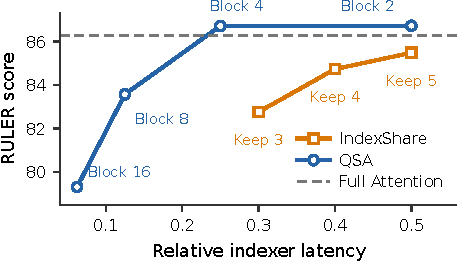
\includegraphics[width=\linewidth]{figs/qsa_latency_ablation.pdf}
        \caption{Compression strategies.}
        \label{fig:qsa-compression-ratio}
    \end{subfigure}
    \hfill
    \begin{subfigure}[t]{0.45\linewidth}
        \centering
        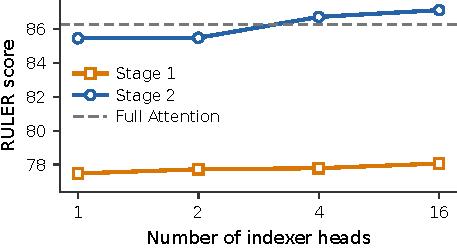
\includegraphics[width=\linewidth]{figs/qsa_head_ablation.pdf}
        \caption{Indexer head configurations.}
        \label{fig:qsa-indexer-heads}
    \end{subfigure}
    \caption{Architecture ablations of QSA on RULER. 
    (a) QSA performance with different micro-block sizes;
    ``Keep $x$'' indicates the number of IndexShare indexer layers retained for computation. 
    (b) Performance with different numbers of indexer query heads after dense distillation and sparse training.}
    \label{fig:qsa-architecture-ablation}
\end{figure}

\paragraph{Architecture Ablation.}
% Intro
We conduct architectural ablations of QSA at the 35B-A3B scale, focusing on the compression ratio and the number of indexer heads.
% Metric
As shown in Fig.~\ref{fig:qsa-architecture-ablation}, we use RULER~\citep{hsieh2024ruler} scores at sequence lengths up to 1M as the evaluation metric.
% Stage1&Stage2
All experiments are evaluated using the CPT models obtained after stage 2 sparse training.

% Compression ratio
For the compression-ratio ablation, we evaluate QSA with different micro-block sizes.
% IndexShare
We additionally include training-aware IndexShare~\citep{bai2026indexcache} as a baseline, 
which reduces indexing overhead by uniformly sharing top-$K$ indices across adjacent full-attention layers in the hybrid model.
% IndexShare in Hybrid
In Fig.~\ref{fig:qsa-architecture-ablation}(a), we report the RULER performance of both approaches against their estimated reductions in indexer latency.
% report
QSA matches the full-attention baseline at a relative indexer latency of 0.25, whereas IndexShare remains below the baseline at 0.5.
For IndexShare, 0.5 denotes sharing a single index across two full-attention layers separated by three GDN layers.
% Hybrid better solution
This result highlights the advantage of intra-layer compression in hybrid architectures, where cross-layer index sharing can be limited by low inter-layer similarity.


% MQA Indexer Head Num
The number of query heads directly affects indexer efficiency, particularly during the prefill stage.
% setting
We therefore evaluate MQA indexers with varying numbers of query heads on RULER, as shown in Fig.~\ref{fig:qsa-architecture-ablation}(b).
% Stage1 & Stage2
After dense initialization, directly applying the indexer for sparse attention leads to a clear performance drop. 
A brief period of joint training allows the backbone to adapt to the sparse attention pattern and recover to the full-attention level.
% Result
The results show that QSA maintains performance with only a small number of indexer query heads,
far fewer than used in the core attention module.
% Efficient
To balance inference speed and accuracy,
we ultimately adopt 4 query heads as a lightweight indexer configuration.

\paragraph{Efficiency Analysis.}
% Seq-level Compression
By compressing the key sequence with a ratio of $r$, QSA reduces indexer complexity from $O(n^2)$ to $O(n^2/r)$, which yields substantial efficiency gains on long sequences.
% Indexer
For the indexer, sequence compression directly reduces the computation of MQA logits and top-$k$ selection,
yielding a speedup comparable to the compression ratio.
As shown in Fig.~\ref{fig:qsa-efficiency}(a,b), this substantially reduces inference costs on long sequences, where the indexer becomes a major bottleneck.


\begin{figure}[t]
    \centering
    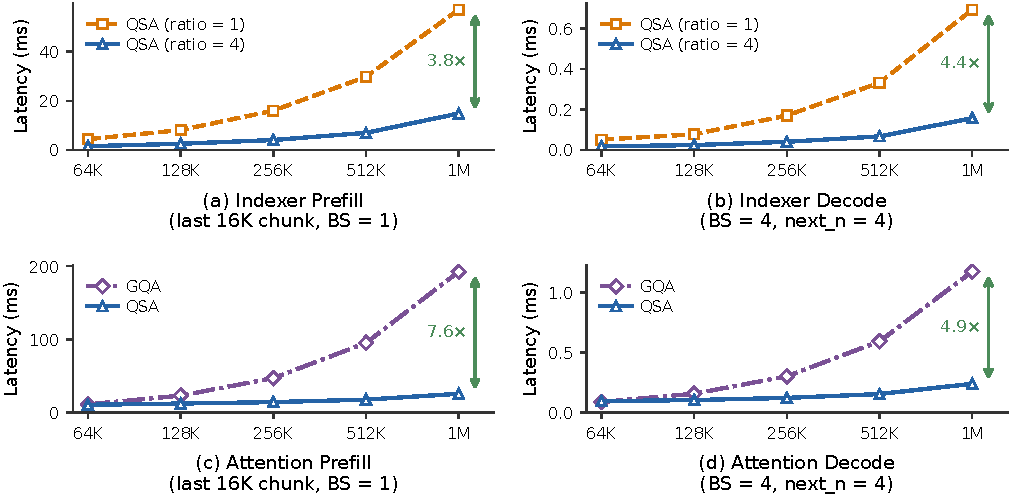
\includegraphics[width=\linewidth]{figs/qsa_efficiency_2x2_b4.pdf}
    \caption{Kernel-level latency of QSA across context lengths during prefill
    and decode. Panels
    (a,b) compare indexer latency under different compression ratios, while
    panels (c,d) compare kernel-level attention latency between dense GQA and
    QSA, including both the indexer and sparse core attention. Chunked prefill
    uses a 16K-token chunk with batch size 1; decode uses batch size 4 and
    \texttt{next\_n}$=4$, corresponding to three MTP prediction steps. Arrows
    indicate speedups at a context length of 1M.}
    \label{fig:qsa-efficiency}
\end{figure}

% Attention
We further evaluate the kernel-level speedup of QSA, accounting for both the indexer cost and sparse core attention computation.
% Setting
For the dense-attention baseline, we use the paged GQA implementation provided by FlashInfer~\citep{ye2025flashinfer}.
Prefill is evaluated under a chunked-prefill setting, while decode includes three additional MTP steps.
% Figure
As shown in Fig.~\ref{fig:qsa-efficiency}(c,d), QSA provides speedups from a context length of 64K, with increasingly larger gains as the sequence length grows.
% conclusion
At a context length of 1M, QSA achieves $7.6\times$ and $4.9\times$ attention-module speedups for prefill and decode, respectively, demonstrating its scalability for long-context inference.
